\documentclass[xcolor=dvipsnames]{beamer}
% Sandpiles
\mode<presentation>
\usetheme{silab} 
\usecolortheme{silab}

\usepackage{listings}
\usepackage{pxfonts}

% Show Date in title
\def\showtitledate{}
%\def\fancystyle{}
%\def\showshorttitle{}


% Some color definitions
\definecolor{mygray}{gray}{.75}
\definecolor{titlegray}{gray}{.35}
\definecolor{lightgray}{gray}{.85}
\definecolor{topgray}{gray}{.85}
\definecolor{myblue}{rgb}{0.8, 0.85, 1}
\definecolor{topblue}{rgb}{0.68, 0.68, 0.88}
\definecolor{visblack}{rgb}{0.0, 0.0, 0.0}

% Boxes
\setbeamercolor{uppercol}{fg=black,bg=myblue}
\setbeamercolor{lowercol}{fg=black,bg=mygray}

\usepackage[english]{babel}
\usepackage[utf8]{inputenc}
\usepackage[T1]{fontenc}
\usepackage{graphicx}
\usepackage{amsmath,commath,amsfonts,amssymb,mathtools}
\usepackage{pgf}
\usepackage[autostyle=true]{csquotes}
\usepackage{IEEEtrantools}
\usepackage[varg]{txfonts}
\usepackage{hyperref}
\usepackage{xcolor}
\usepackage[table-format=1.4, separate-uncertainty=false]{siunitx}
\usepackage{fancyhdr}
\usepackage{colortbl}
\usepackage{geometry}
\usepackage{caption}
\usepackage{siunitx}
\usepackage{verbatim}
\usepackage{subfigure}
\usepackage{booktabs}
\usepackage{empheq}
\usepackage{animate}
\usepackage{float}
\usepackage{pdfpages}
\usepackage{multirow}
\usepackage{bigdelim}
\usepackage{floatflt}
\usepackage{scalerel}
\usepackage{tikz}
\graphicspath{{./pics/}{./gifs/}{../analysis/avalanche_formations/}{../analysis/moment_analysis/plots/}
              {../analysis/naive_fits/}}
%\usepackage{ubonn-biblatex}
\usepackage[sorting=none, natbib=true, style=numeric]{biblatex}


\addto{\captionsenglish}{\renewcommand*{\figurename}{Fig.}}
\setbeamertemplate{caption}[numbered]

\newcommand*\widefbox[1]{\fbox{\hspace{2em}#1\hspace{2em}}}
\newcommand{\myitemsep}{\setlength\itemsep{0.33cm}}
\newcommand{\mysubitemsep}{\setlength\itemsep{0.22cm}}

\newcommand{\backupbegin}{
    \newcounter{finalframe}
    \setcounter{finalframe}{\value{framenumber}}
}
\newcommand{\backupend}{
    \setcounter{framenumber}{\value{finalframe}}
}

% Coding stuff
\lstset{language=python, numbers=left, numberstyle=\tiny, showstringspaces=false,
    aboveskip=10pt, frame=leftline}

% No stupid navigation bar
\beamertemplatenavigationsymbolsempty

\useinnertheme{rectangles}
%\setbeamertemplate{navigation symbols}{}

\title[Sandpiles]{Cellular Automata for Sandpiles}
\subtitle{An Example of Self-organized criticality}
\author[M. Frohne \& P. Wolf]{Markus Frohne\\ \texttt{\textcolor{gray}{markusfrohne@uni-bonn.de}}\\
        \vspace{0.33cm} Pascal Wolf\\ \texttt{\textcolor{gray}{pwolf@uni-bonn.de}}}
\date{March 15$^\text{th}$, 2018}

\addbibresource{../report/refs.bib}

\newcommand{\fplus}[1][black]{%
    \tikz\draw[#1,line width=2pt] (0,0) -- (0.25,0)(0.125,0.125) -- (0.125,-0.125);
}

\newcommand{\fminus}[1][black]{%
    \tikz\draw[#1,line width=2pt] (0,0) -- (0.25,0);
}

\begin{document}
    
    \begin{frame}
        \titlepage
    \end{frame}
    
    \begin{frame}{Outline of talk}
        \begin{itemize}
            \myitemsep
            \item Motivation
            \item {Theory
                \vspace{0.22cm}
                \begin{itemize}
                    \mysubitemsep
                    \item[$\bullet$] Self-organized criticality (\textbf{SOC}), cellular automata
                    \item[$\bullet$] The \texttt{Bak-Tang-Wiesenfeld} (\textbf{BTW}) and custom model
                \end{itemize}}
            \item {Simulation
                \vspace{0.22cm}
                \begin{itemize}
                    \mysubitemsep
                    \item[$\bullet$] Visualization of simulated data
                \end{itemize}}
            \item {Analysis 
                \vspace{0.22cm}
                \begin{itemize}
                    \mysubitemsep
                    \item[$\bullet$] Methods
                    \item[$\bullet$] Results
                    \item[$\bullet$] Discussion \& Comparison
                \end{itemize}}
            \item Summary
        \end{itemize}
    \end{frame}
    
    {\usebackgroundtemplate%
        {%
            
\includegraphics[width=\paperwidth,height=\paperheight]{bkg1.pdf}%
        }
        \begin{frame}
            \centering \Huge \color{ublue} Motivation
            \thispagestyle{empty}
            \addtocounter{framenumber}{-1}
        \end{frame}
    }
    
    \begin{frame}{Motivation}
        \begin{itemize}
            \item Critical phenomena are studied widely
            \item The Ising model% consists of a collective of magnetic moments represented by spins $\vec{s}$
                                 % on a lattice:
            \begin{itemize}
                \item Main tunable model parameter: temperature $T$
                \item Phase transition at critical temperature $T_{\mathrm{c}}$
                \item Cluster formation with characteristic properties
            \end{itemize}
        \end{itemize}
        \begin{figure}[htb]
            \centering
            \animategraphics[width=0.45\linewidth, loop, autoplay]{10}{ising-}{0}{199}
            \caption{Ising model cluster formation around the critical temperature.}
            \label{fig:}
        \end{figure}
    \end{frame}

    \begin{frame}{Motivation}
        \begin{columns}[t]
            \begin{column}{0.6\linewidth}
                \begin{itemize}
                    \item Ising model needs tunable 
                    \item Phenomena in nature
                        \begin{itemize}
                            \item landslides
                            \item earthquakes
                            \item forest fires
                            \item seacoasts
                            \item \emph{sandpiles}
                        \end{itemize}
                \end{itemize}
                \begin{itemize}
                    \item Different types of critical phenomena
                        \begin{itemize}
                            \item \enquote{standard} critical phenomena
                            \item \enquote{self-organized} critical phenomena
                        \end{itemize}
                \end{itemize}
            \end{column}
            \begin{column}{0.4\linewidth}
                \begin{figure}[htb]
                    \centering
                    \includegraphics[width=0.8\linewidth]{landslide}
                    \caption{A rock landslide in Guerrero, Mexico.\\
                             \footnotesize from: Wikimedia Commons, \emph{File:Slide-guerrero1.JPG}}
                    \label{fig:}
                \end{figure}
            \end{column}
        \end{columns}
    \end{frame}

    
    {\usebackgroundtemplate%
        {%
            
\includegraphics[width=\paperwidth,height=\paperheight]{bkg1.pdf}%
        }
        \begin{frame}
            \centering \Huge \color{ublue} Theory
            \thispagestyle{empty}
            \addtocounter{framenumber}{-1}
        \end{frame}
    }
    
    {\usebackgroundtemplate%
        {%
            
\includegraphics[width=\paperwidth,height=\paperheight]{bkg1.pdf}%
        }
        \begin{frame}
            \centering \Huge \color{ublue} Simulations \\ \Large Visualization of data and analysis methods
            \thispagestyle{empty}
            \addtocounter{framenumber}{-1}
        \end{frame}
    }
    
    \begin{frame}{Sandpile dynamics -- Avalanche evolution}
        \begin{figure}[h]
            \captionsetup{width=0.9\textwidth}
            \centering
            \only<1>{
            \subfigure[BTW model]{\animategraphics[width=0.475\textwidth, loop, autoplay]{10}{btw_center_}{1}{250}}
            \subfigure[Custom model]{\animategraphics[width=0.475\textwidth, loop, autoplay]{10}{custom_center_}{1}{250}}
            \caption{Avalanche evolution in a 2D sandbox of length 50 (\textbf{center} drives)}}
            \only<2>{
            \subfigure[BTW model]{\animategraphics[width=0.475\textwidth, loop, autoplay]{10}{btw_random_}{1}{250}}
            \subfigure[Custom model]{\animategraphics[width=0.475\textwidth, loop, autoplay]{10}{custom_random_}{1}{250}}
            \caption{Avalanche evolution in a 2D sandbox of length 50 (\textbf{random} drives)}}
        \end{figure}
    \end{frame}
    
    \begin{frame}{Sandpile dynamics -- Avalanche formations}
        \begin{figure}[h]
            \captionsetup{width=0.9\textwidth}
            \begin{center}
                \only<1>{
                \subfigure[2D]{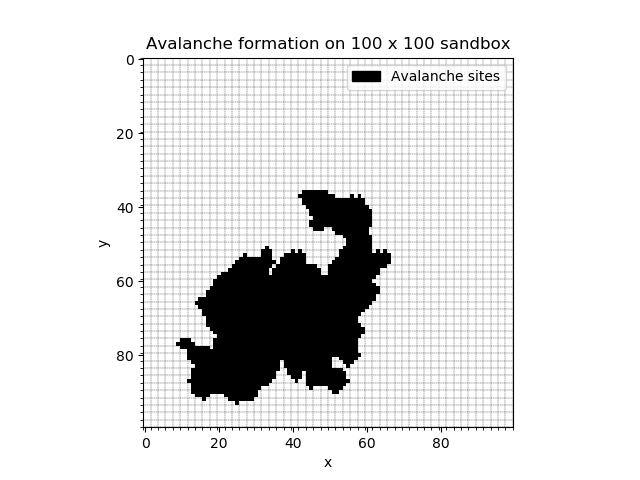
\includegraphics[width=0.475\textwidth]{Avalanche_2d_btw_1.png}}
                \subfigure[3D]{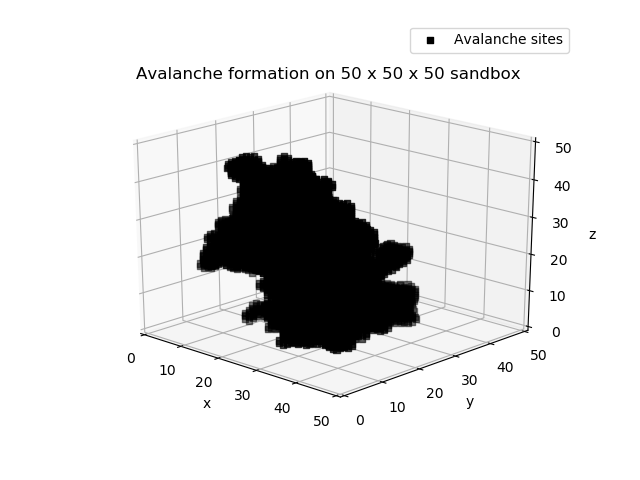
\includegraphics[width=0.475\textwidth]{Avalanche_3d_btw_6.png}}
                \caption{Avalanche formation in the BTW model.}}
                \only<2>{
                \subfigure[2 D]{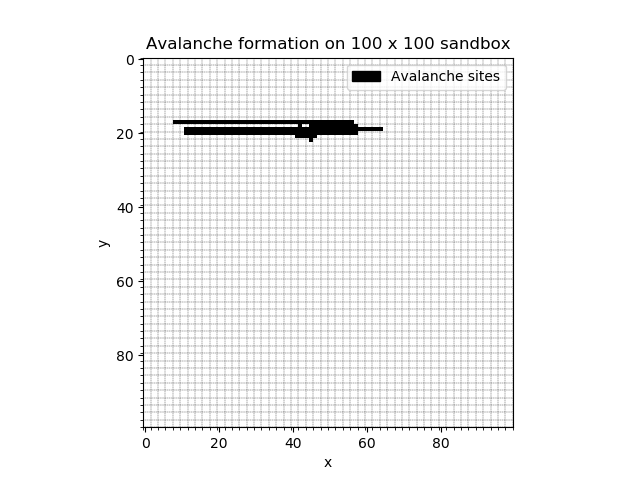
\includegraphics[width=0.475\textwidth]{Avalanche_2d_custom_11.png}}
                \subfigure[3 D]{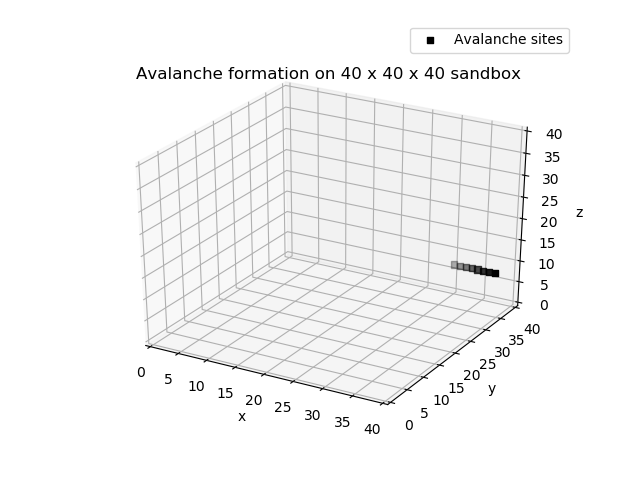
\includegraphics[width=0.475\textwidth]{Avalanche_3d_custom_4.png}}
                \caption{Avalanche formation in the custom model.}}
            \end{center}
        \end{figure}
    \end{frame}
    
    
    {\usebackgroundtemplate%
        {%
            
\includegraphics[width=\paperwidth,height=\paperheight]{bkg1.pdf}%
        }
        \begin{frame}
            \centering \Huge \color{ublue} Analysis
            \thispagestyle{empty}
            \addtocounter{framenumber}{-1}
        \end{frame}
    }
    
    \begin{frame}{Analysis method -- Naive fit}
        \begin{itemize}
            \item {Straight line fit for initial verification of power-law scaling behavior
                \begin{align*}
                P^{(Y)}(y) \propto y^{-\rho}
                \end{align*}
                }
            \item {$P^{(Y)}(y)$ deviates from linear trend due to \textit{finite size effects}:\\
                   $\Rightarrow$ \textit{moment analysis}}
        \end{itemize}
        \begin{figure}[h]
            \captionsetup{width=\textwidth}
            \centering
            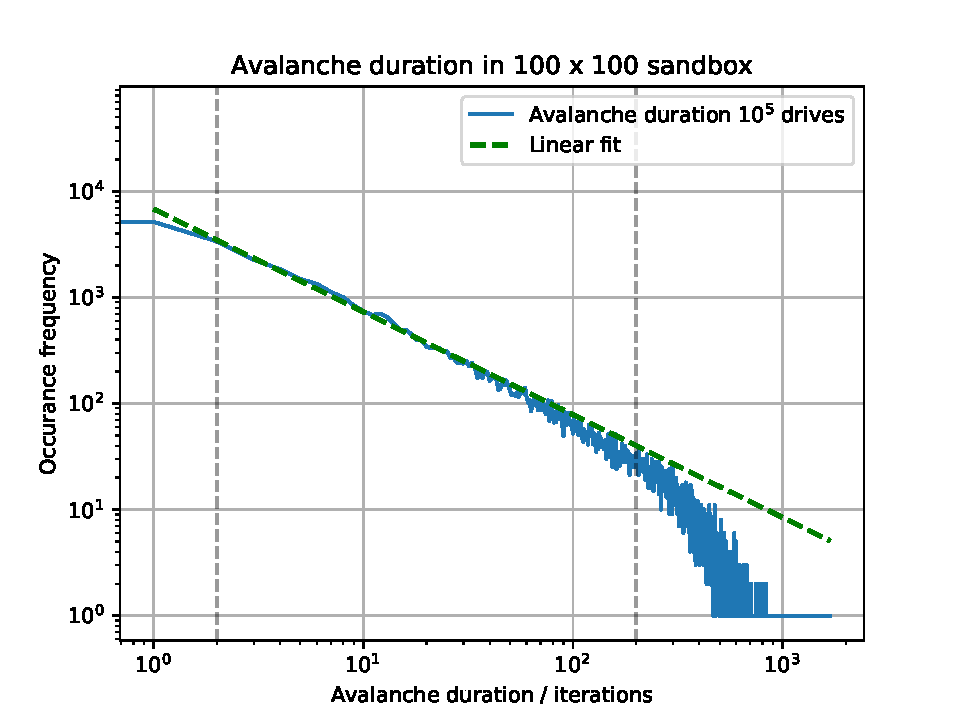
\includegraphics[width=0.51\textwidth]{naive_fit.pdf}
            \caption{Power law scaling behavior of avalanche duration of the BTW model.}
        \end{figure}
    \end{frame}
    
    \begin{frame}{Analysis method -- Moment analysis}
        \begin{itemize}
            \myitemsep
            \item {Define the so-called $n^{\mathrm{th}}$ \textit{moment} of the observable $y$ by
                \begin{align*}
                \left\langle y^n \right\rangle = \int_{0}^{\infty} dy\ y^n P^{(y)}(y)
                \end{align*}
                where $P^{(y)}$ is the PDF of $y$.
            }
            \item {For $L \to \infty$ the following relation holds:
                \begin{align*}
                \left\langle y^n \right\rangle \propto L^{K\left(1 + n - \rho \right)} \qquad \text{with}
                                                                \qquad K\left(1 + n - \rho \right) \equiv \sigma_n 
                \end{align*}
                where $K,\ \rho$ is the set of scaling exponents of the observable $y$. Taking the logarithm,
                this relation exhibits a linear trend with slope $\sigma_n$.
            }
            \item {Determination scaling exponents of the $1^{\text{st}}$ and $2^{\text{nd}}$ moment $\sigma_1$ and
                   $\sigma_2$ allows for the calculation of the set of critical exponents $K,\ \rho$:
                \begin{align*}
                K = \sigma_2 - \sigma_1 \quad , \quad \rho = \frac{2\sigma_2 - 3\sigma_1}{\sigma_2 - \sigma_1} 
                \end{align*} 
            }
        \end{itemize}
    \end{frame}
    
    \begin{frame}{Analysis method -- Moment analysis}
        \begin{itemize}
            \myitemsep
            \item {General approach of moment analysis:
                \begin{itemize}
                    \mysubitemsep
                    \item[$\bullet$] Simulate $R$ samples for $N$ lattice sizes $L_N$, record PDF of observables and
                                     calculate $\left\langle y^1 \right\rangle,\ \left\langle y^2 \right\rangle$
                    \item[$\bullet$] Draw \textit{random} bootstrap sample from $\left\langle y^1 \right\rangle_R,
                                     \ \left\langle y^2 \right\rangle_R$ for each $L_N$
                    \item[$\bullet$] Calculate covariance matrix for each bootstrap (\textbf{double bootstrap})
                    \item[$\bullet$] Linear fit within each bootstrap sample to calculate and store $K,\ \rho$
                    \item[$\bullet$] Estimate uncertainties by the standard deviation of $K,\ \rho$ from all bootstraps
                \end{itemize}
            }
            \item[$\Rightarrow$] {Actual numbers for analysis in 2 and 3 dimensions:
                \begin{itemize}
                    \mysubitemsep
                    \item[$\bullet$] $R = 10$
                    \item[$\bullet$] $N = R$ with $L_N \in \{10, 20, 30, 40, 50, 60, 70, 80, 90, 100\}$
                \end{itemize}
            }
        \end{itemize}
    \end{frame}
    
    \begin{frame}{Analysis method -- Moment analysis}
        \begin{figure}[htp]
            \centering
            \only<1>{
            \subfigure[BTW]{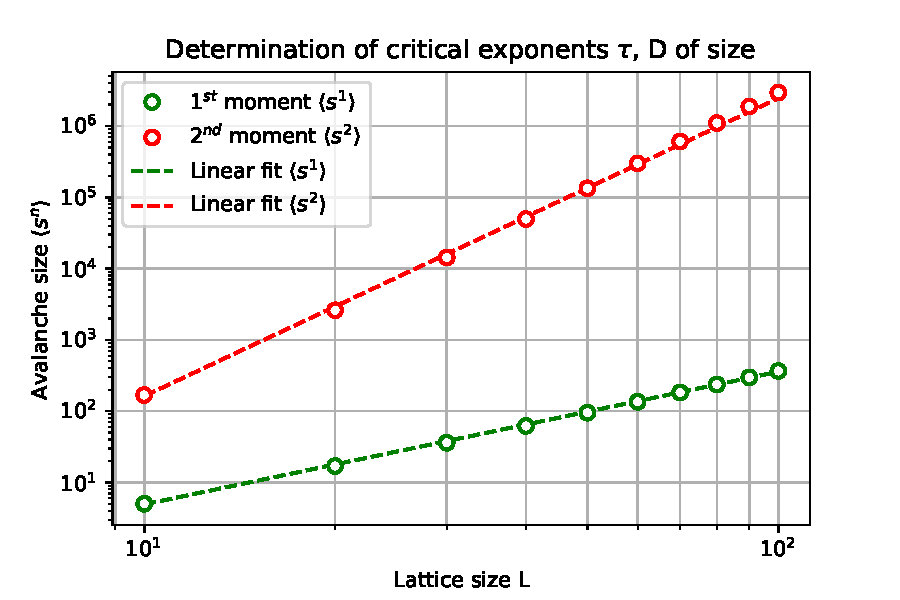
\includegraphics[width=0.475\textwidth]{moment_analysis_size_2d_btw_fit.pdf}}
            \subfigure[Custom]{\includegraphics[width=0.475\textwidth]{{moment_analysis_size_2d_custom_crit_%
                                                                        slope_7_fit.pdf}}}
            \caption{$1^{\mathrm{st}}$ and $2^{\mathrm{nd}}$ moments of one \textit{random} bootstrap sample for
                     avalanche \textbf{size} and overall best linear fit in 2D.}
            }
            \only<2>{
            \subfigure[BTW]{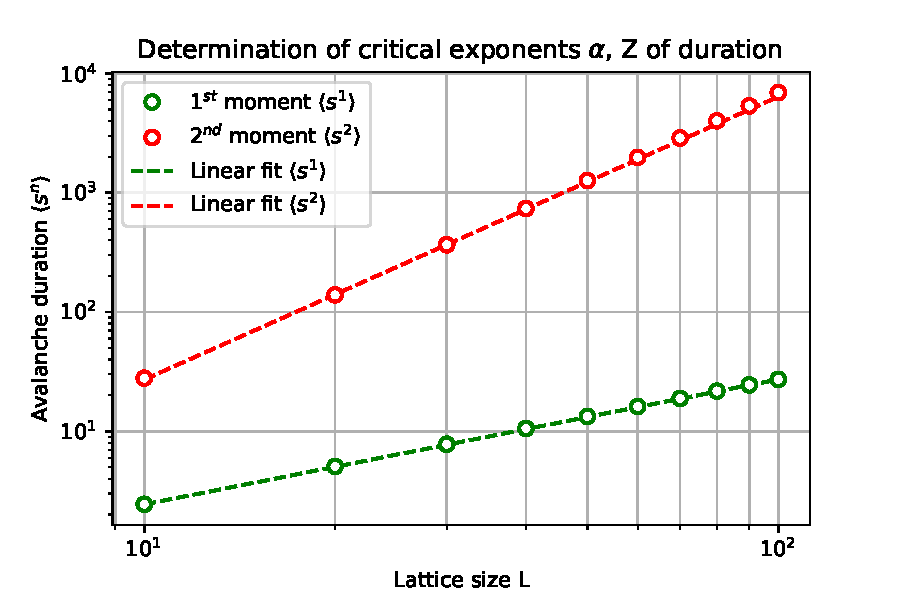
\includegraphics[width=0.475\textwidth]{moment_analysis_duration_2d_btw_fit.pdf}}
            \subfigure[Custom]{\includegraphics[width=0.475\textwidth]{{moment_analysis_duration_2d_custom_crit_slope_%
                                                                        7_fit.pdf}}}
            \caption{$1^{\mathrm{st}}$ and $2^{\mathrm{nd}}$ moments of one \textit{random} bootstrap sample for
                     avalanche \textbf{size} and overall best linear fit in 2D.}
            }
            \only<3>{
            \subfigure{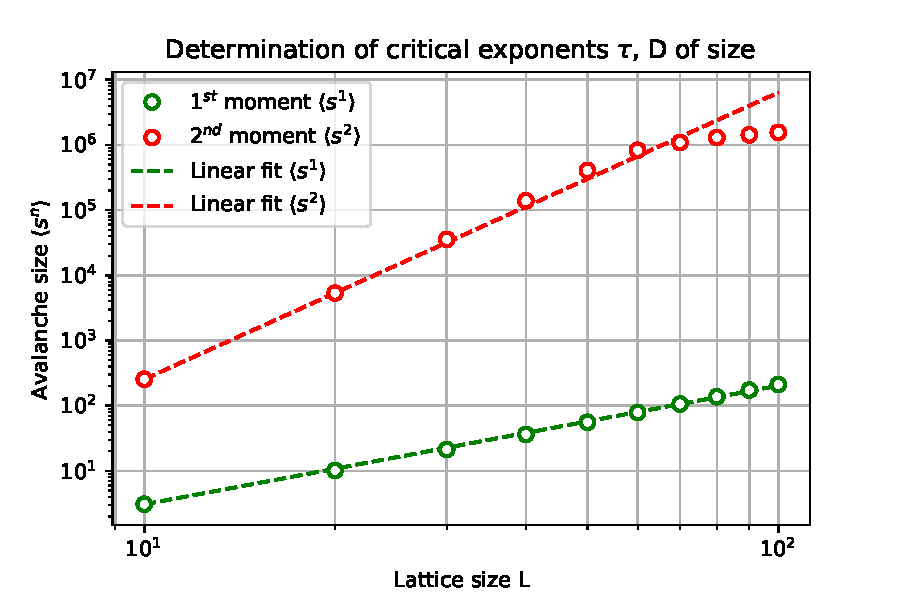
\includegraphics[width=0.475\textwidth]{moment_analysis_size_3d_btw_fit.pdf}}
            \subfigure{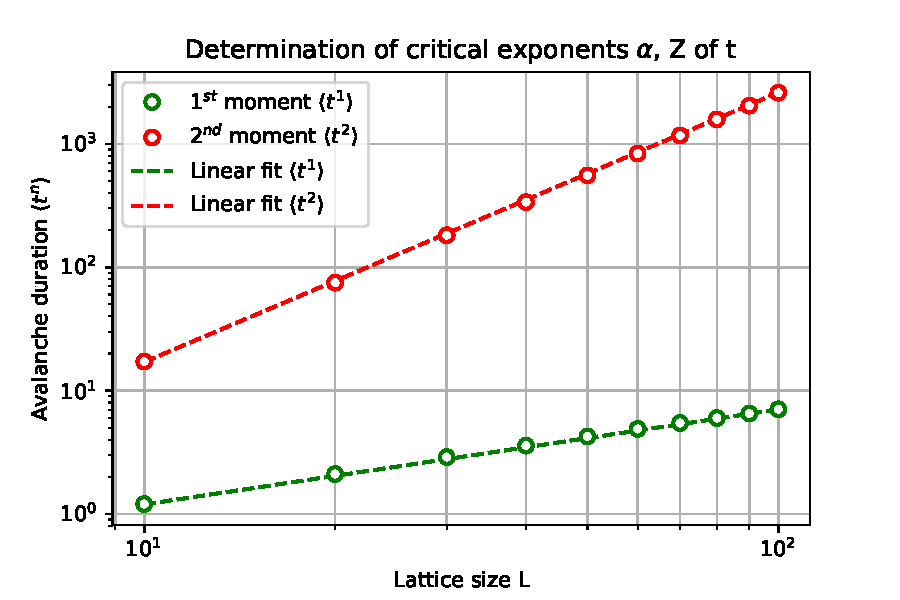
\includegraphics[width=0.475\textwidth]{moment_analysis_duration_3d_btw_fit.pdf}}
            \caption{$1^{\mathrm{st}}$ and $2^{\mathrm{nd}}$ moments of one \textit{random} bootstrap sample for
                     avalanche \textbf{size} and overall best linear fit in 3D.}
            }
        \end{figure}
    \end{frame}
    
    \begin{frame}{Analysis results -- Moment analysis}
        \renewcommand{\arraystretch}{1.15}
        \begin{table}[htb]
            \centering
            \begin{tabular}{llSScSScSS}
            \toprule
            & \multirow{2}{*}{Model} & \multicolumn{2}{c}{Size} && \multicolumn{2}{c}{Duration} &&
                                                                   \multicolumn{2}{c}{Area} \\
            \cmidrule{3-4} \cmidrule{6-7} \cmidrule{9-10}
            && {$\tau$} & {$D$} && {$\alpha$} & {$Z$} && {$\kappa$} & {$T$} \\
            \cmidrule{2-10}
            \cmidrule{2-10}
            \hspace{-15px}\ldelim\lbrace{3}{0mm}[$2$D] &
            $\mathrm{BTW}$ & 1.19(9) & 2.3(2) && 1.21(2) & 1.34(3) && 1.23(7) & 1.9(2) \\
            & $\mathrm{CST}_{\mathrm{C}5}$ & 1.3(2) & 1.6(2) && 1.2(2) & 0.7(2) && 1.3(2) & 0.8(2) \\
            & $\mathrm{CST}_{\mathrm{C}7}$ & 1.4(2) & 1.6(4) && 1.3(1) & 0.81(8) && 1.4(1) & 1.0(1) \\
            \midrule
            \hspace{-15px}\ldelim\lbrace{2}{0mm}[$3$D] &
            $\mathrm{BTW}$ & 1.3(1) & 2.5(3) && 1.45(3) & 1.41(6) && 1.4(3) & 2.6(7) \\
            & $\mathrm{CST}_{\mathrm{C}5}$ & 1.23(1) & 1.99(2) && 1.29(1) & 1.17(1) && 1.29(1) & 1.43(1)\vspace{2px}\\
            \bottomrule
            \end{tabular}
            \caption{Scaling exponents for avalanche size, duration and area.}
            \label{tab:scalingExp}
        \end{table}
    \end{frame}

\end{document}